\subsubsection{Windows 10}

Nach dem Boot wird der Raspberry Pi Zero als "`Serielles USB-Ger�t"' erkannt und keine korrekten Treiber installiert. Dies muss manuell erfolgen. Dazu l�dt man sich zuerst den zertifizierten Treiber "`Acer Incorporated. - Other hardware - USB Ethernet-RNDIS Gadget"' von der Microsoft Homepage herunter \url{http://download.windowsupdate.com/msdownload/update/driver/drvs/2012/12/20342322_4b9970e3174b23b5cb2371af0837f939a71271ea.cab}. Die ben�tigten Dateien sind in der komprimierten CAB-Datei enthalten. Durch einen Doppelklick auf der Datei kann der Inhalt dargestellt werden. Mit der rechten Maustaste und dem Kontexmen� k�nnen die Dateien z.~B. nach \path{c:\Drivers\RNDIS\} extrahiert werden. 

\begin{figure}[ht]
  \centering
  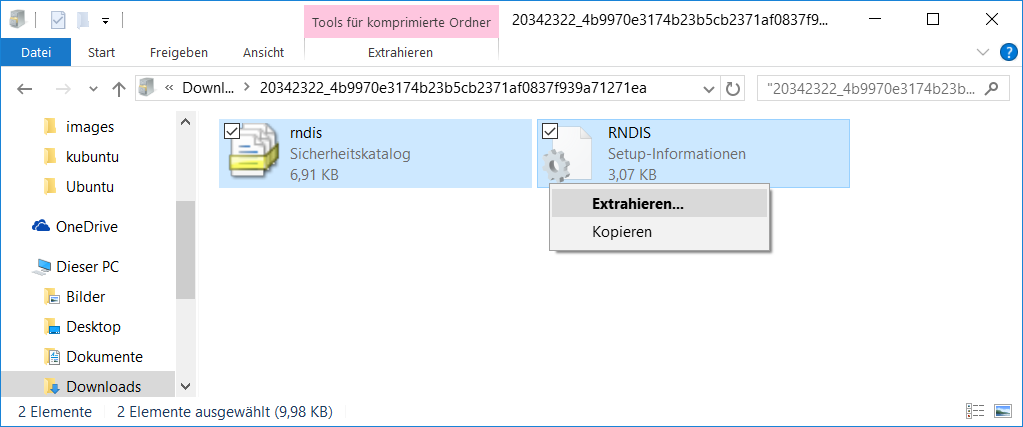
\includegraphics[scale=0.42]{images/OTG_Win10_Install_0.png}
%  \caption{}
  \label{OTG_Win10_Drivers}
\end{figure}

Nun muss der Gr�temanager ge�ffnet werden. Dann �ffnet man das Kontextmen� in dem man die rechten Maustatste am 
"`Serielles USB-Ger�t"' Eintrag dr�ckt. Nun w�hlt man den Men�punkt "`Treiber Software aktualisieren..."' aus. Im folgenden Dialog w�hlt man "`Auf dem Computer nach Treibersoftware suchen"' und dann gibt man das Verzeichnis an in dem die Treiberdaten extrahiert wurden, z.~B. \path{c:\Drivers\RNDIS\}. Zum Schluss sollte der Treiber automatisch erfolgreich installiert werden.\\ 

\begin{figure}[ht]
  \centering
  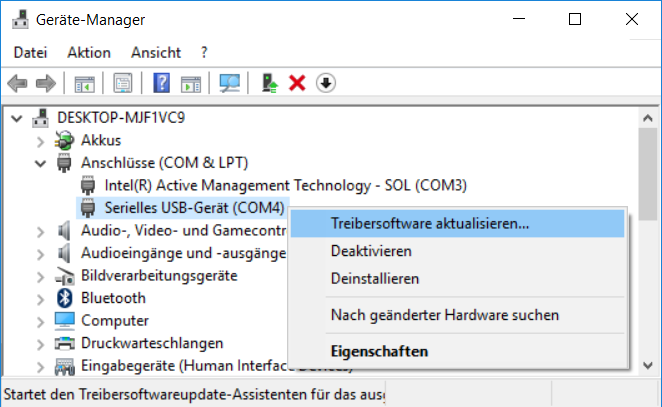
\includegraphics[scale=0.42]{images/OTG_Win10_Install_1.png}
%  \caption{}
  \label{OTG_Win10_Install_1}
\end{figure}

\begin{figure}[ht]
  \centering
  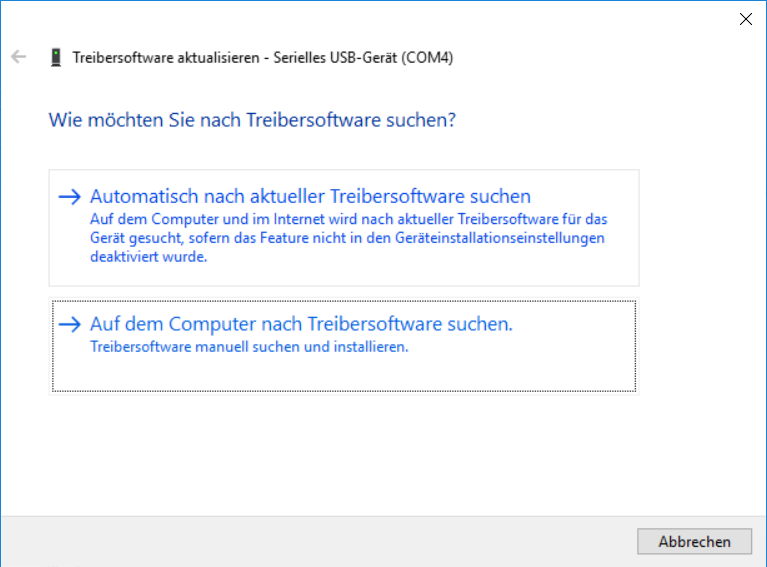
\includegraphics[scale=0.42]{images/OTG_Win10_Install_2.png}
%  \caption{}
  \label{OTG_Win10_Install_2}
\end{figure}  

\begin{figure}[ht]
  \centering
  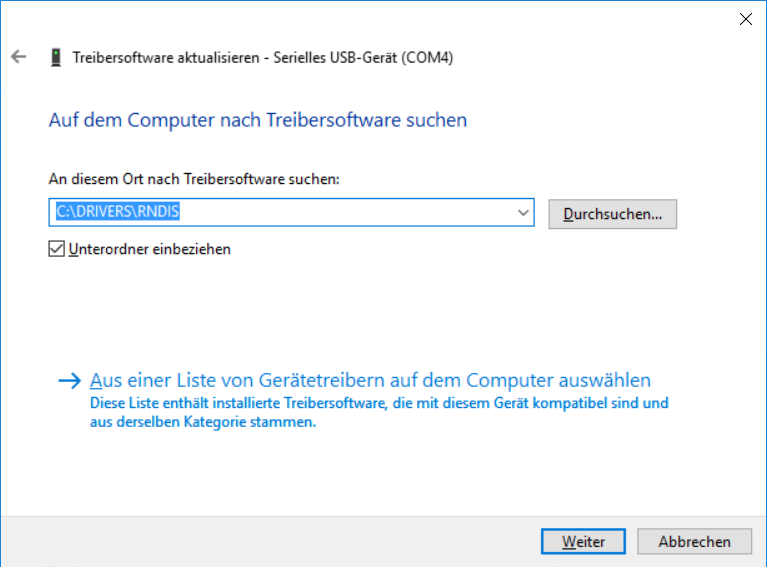
\includegraphics[scale=0.42]{images/OTG_Win10_Install_3.png}
%  \caption{}
  \label{OTG_Win10_Install_3}
\end{figure}  


\begin{figure}[ht]
  \centering
  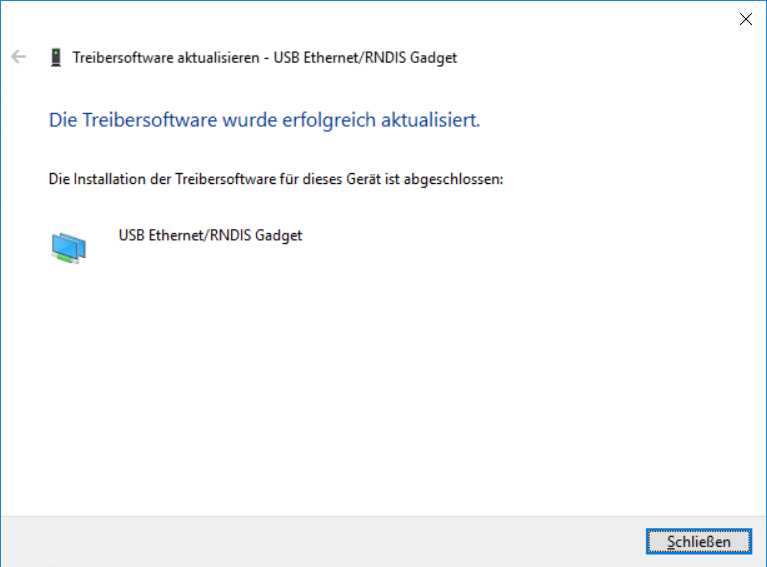
\includegraphics[scale=0.42]{images/OTG_Win10_Install_4.png}
%  \caption{}
  \label{OTG_Win10_Install_4}
\end{figure}  



%%%%%

Damit am Ger�t Internet funktionieren kann, muss das Internet f�r das neue Netzwerk freigegeben werden. Dazu �ffnet man das Einstellungs-Fenster f�r die Netzwerkverbindungen. 

\begin{figure}[ht]
  \centering
  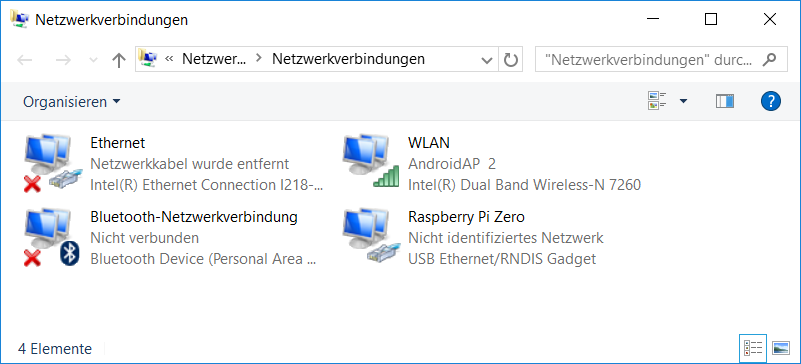
\includegraphics[scale=0.42]{images/OTG_Win10_Netzwerkverbindungen.png}
%	\caption{}
  \label{OTG_Win10_Netzwerkverbindungen}
\end{figure}

Zuerst kann man dem Netzwerkger�t "`USB Ethernet/RNDIS Gadget"' einen neuen Namen geben, z.~B. Raspberry Pi Zero. Nun muss das Netzwerk gesucht werden, das mit dem Internet verbunden ist, z.~B. WLAN. Bei den Eigenschaften zu dem Netzwerk kann der Reiter "`Freigabe"' ausgew�hlt werden. Danach kann man die Einstellung "`Anderen Benutzern im Netzwerk gestatten, diese Verbindung des Computers als Internetverbindung zu verwenden"' aktivieren und bei Heimnetzwerkverbindung kann das Netzwerk "`Raspberry Pi Zero"' ausgew�hlt werden.\\
%Windows 7 legt dann fest, dass die Netzwerkadresse 192.168.137.1 sein muss. Alternativ kann die Verbindung auch zuvor schon auf diese statische IP-Adresse gesetzt werden.\\


%\begin{figure}[ht]
%  \centering
%  \includegraphics[scale=0.42]{images/OTG_Win10_IPv4_1.png}
%  \includegraphics[scale=0.42]{images/OTG_Win10_IPv4_2.png}
%%	\caption{}
%  \label{OTG_Win10_IPv4_12}
%\end{figure}

\begin{figure}[ht]
  \centering
  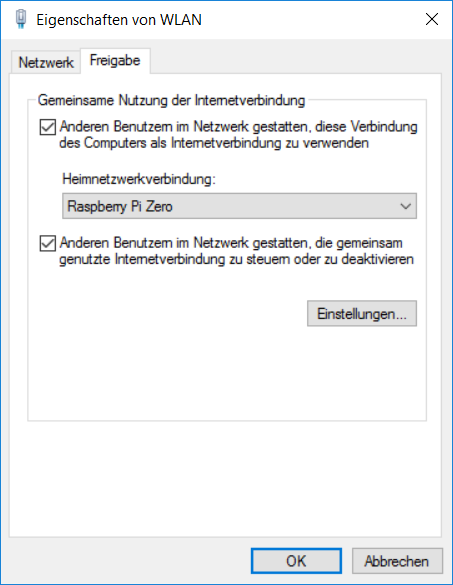
\includegraphics[scale=0.42]{images/OTG_Win10_Inet.png}
%	\caption{}
  \label{OTG_Win10_Inet}
\end{figure}


Nun kann die Verbindung zur Raspberry Pi mit dem Programm Putty und der Adresse "`192.168.137.10"', �ber das SSH-Protokoll hergestellt werden.\\  
Mit dem Befehl "`ping 8.8.8.8"' kann die Internetverbindung getestet werden. Mit dem Befehl "`ping google.com"' kann dann der DNS-Server �berpr�ft werden.   
